\chapter{Introdução}


%-----------------------------------------
%-----------------------------------------
\section{Descrição do Problema}

Em um mundo altamente globalizado e de tecnologias emergentes, empresas se veem na necessidade de modernizarem a si mesmas em face à grande competitividade existente. Grandes, médios, pequenos e micro negócios tiveram de se adequar às demandas dessa nova realidade, sobretudo no que diz a respeito da informatização de processos, com o intuito de lograr rapidez e eficiência. Daí surge a chamada agilidade operacional, a tendência de tornar estes processos dinâmicos e flexíveis.

A Universidade do Estado do Amazonas (UEA) é a maior universidade multicampi do país, sendo composta por vinte e três unidades diferentes, possuindo mais de vinte mil alunos matriculados em sua totalidade. Apesar de ser uma instituição de ensino de grande porte, vários de seus processos internos estão de certa forma defasados, demandando mais recursos humanos que o necessário, consequentemente acarretando em perdas operacionais, e até mesmo monetárias. 

O RU (Restaurante Universitário) é o local encarregado de prover aos alunos, técnicos e professores da instituição refeições diversificadas e de qualidade por um preço acessível ao público, contemplando uma refeição para cada turno do dia: café da manhã pelo turno da manhã, almoço pelo turno da tarde e lanche pelo turno da noite. Para fazer uso do Restaurante Universitário, o aluno deve, primeiramente, emitir uma carteirinha própria da UEA.

Apesar de cumprir o seu objetivo primário, o RU é uma área da universidade tida por grande parte dos alunos como insatisfatória, sobretudo no que vem a ser o seu fluxo de atendimento: o aluno, munido de sua carteirinha de estudante, deve enfrentar longas filas para realizar a compra de um ticket de alimentação, para então novamente enfrentar outra fila, desta vez para obter de fato a sua refeição.

Com isso, perdas notáveis ocorrem no convívio diário dos alunos dentro da universidade. Visto que muitos não conseguem se alimentar em tempo hábil, os discentes que optam por não almoçar vão à sala de aula com fome, minando assim o desempenho que outrora possuiriam caso estivessem bem alimentados. Outra parte dos usuários do local dedica um esforço a obter comida de outras fontes, uma alternativa que acaba sendo monetariamente cara, se comparada ao preço convidativo do Restaurante Universitário, ou até mesmo maléfica para a saúde, caso o aluno opte por comer fast-food ou comidas pré-prontas.

Além dos alunos, parte do corpo docente e dos técnicos gerais da universidade também frequenta o restaurante, agravando ainda mais a situação já precária. Felizmente, uma solução para esta problemática está em andamento, que é o desenvolvimento de uma aplicativo para dispositivos móveis para dar suporte ao RU.

No entanto, surge um desafio na implementação desta solução: garantir segurança nas informações armazenadas. Segundo dados de um estudo da Roland Berger, empresa alemã de consultoria estratégica, em 2021 o Brasil foi o 5° maior país a sofrer ataques cibernéticos \cite{SecurityReport}, sobretudo ataques de ransomware, modalidade de ataque que consiste em tornar as vítimas reféns ao demandar o pagamento de um resgate para recobrar o acesso aos seus próprios dados.  O ranking National Cyber Security Index \cite{NCSI}, um índice global que mede o preparo e a prontidão dos países para lidar com ciberataques, figura o Brasil na 68° com um índice de cibersegurança de 51.95 (Figura \ref{fig:ncsi}); em comparação com a Grécia, que ocupa o primeiro lugar com ranking de 96.10, observamos uma enorme disparidade.

\begin{figure}
    \centering
    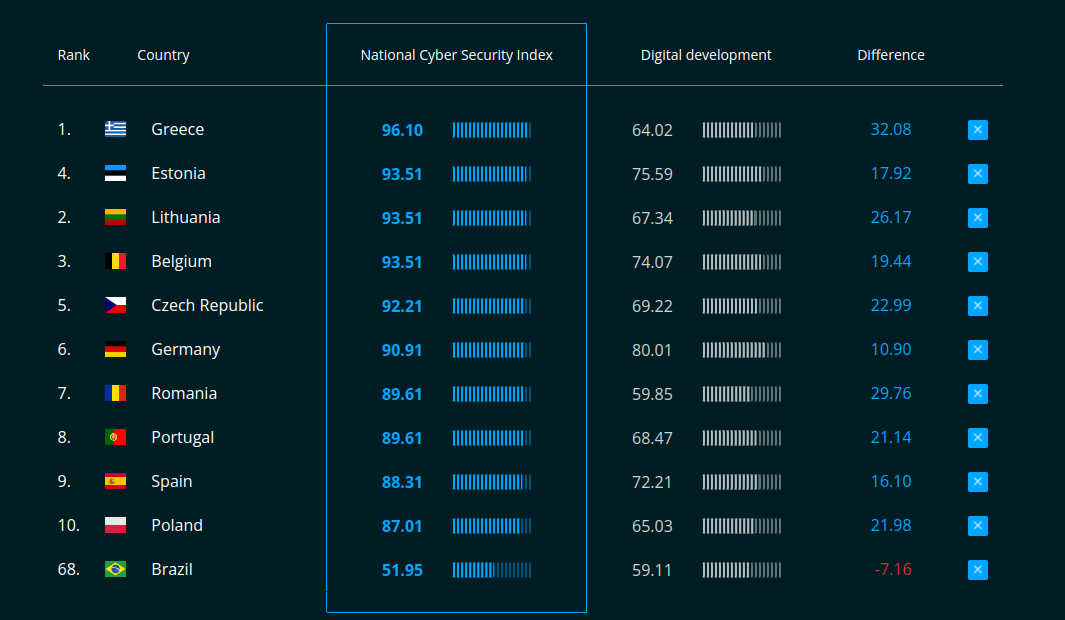
\includegraphics[width=1\textwidth]{img/Cap1/NCSI ranking.png}
    \caption{Ranking NCSI de cibersegurança global \cite{NCSI}}
    \label{fig:ncsi}
\end{figure}

Casos como o ataque de ransomware sofrido pelas lojas Renner \cite{TheHack} nos reforçam a importância de investir em segurança ao se desenvolver um software. As consequências de um ataque deste tipo não são apenas financeiras, mas também operacionais, resultando em indisponibilidade em sistemas de informação. A depender da aplicação, esta indisponibilidade pode ser fatal, afetando vidas humanas. Um dos maiores casos de ciberataque da história afetou diversos hospitais de um serviço de saúde dos Estados Unidos, minando os atendimentos e visualização de dados de pacientes, obrigando os colaboradores a recorrerem ao uso de papel e caneta \cite{NBCNews}. E este cenário tende a piorar: análises de \cite{CheckPointResearch} indicam que a taxa de ciberataques globais sofreu um aumento de 42\% no ano de 2022.
 
Incidentes em que há perda de posse de informações privadas, casos de roubo ou adulteração de dados sensíveis (que muitas vezes passam despercebidos pois são de difícil identificação) e episódios de indisponibilidade de dados podem ser evitados pelo uso da tecnologia Blockchain. A Blockchain possibilita contornar esses e outros problemas de segurança capazes de acometer um sistema computacional devido às suas particularidades. Considerada por diversos especialistas como uma tecnologia revolucionária e disruptiva devido ao seu enorme potencial \cite{Ejeke2022}, é uma das precursoras da chamada Web 3.0, uma evolução da rede mundial de computadores com foco na descentralização da informação.

A Blockchain é uma tecnologia que consiste em um conjunto de registros, os blocos, que são encadeados por meio de criptografia. Funciona como uma espécie de livro-razão: operações efetuadas na rede, as chamadas transações, são registradas e validadas de tempos em tempos. Após aproximadamente dez minutos essas transações são coletadas e agregadas em um único bloco, que por sua vez passa então por um processo de validação, sendo finalmente anexado no final da Blockchain, formando uma ligação com o último bloco armazenado anteriormente armazenado. Esse processo de validação de bloco se chama mineração e é necessário para garantir que os dados lá armazenados sejam íntegros e fidedignos à realidade. Usando a Blockchain como um repositório de dados conseguimos implementar um sistema seguro e à prova de ataques.


% \newpage %%
%-----------------------------------------
%-----------------------------------------
\section{Objetivos}

\subsection{Objetivo Geral}

O objetivo deste trabalho é desenvolver um sistema de registros (\emph{logs}) baseado na tecnologia Blockchain para o aplicativo Carteira Digital do Restaurante Universitário da UEA, fornecendo assim suporte à auditorias e análises do funcionamento do sistema em face à utilização por parte do usuário.

\subsection{Objetivo Específico}
O objetivo geral pode ser decomposto nos seguintes itens:
\begin{enumerate}
    \item Desenvolver um sistema de suporte a processos de auditoria por meio de uma API para o aplicativo Carteira Digital do Restaurante Universitário da UEA;
    \item Implementar comunicação com a Blockchain Ethereum e utilizá-la para garantir segurança à aplicação;
    \item Criar \emph{endpoints} na aplicação para tornar possível registro e leitura de informações de uso do sistema;
    \item Realizar integração entre o sistema desenvolvido e o \emph{back-end} do aplicativo Carteira Digital do Restaurante Universitário da UEA;
    \item Tornar possível a realização de auditorias no sistema.
\end{enumerate}


%-----------------------------------------
%-----------------------------------------
\section{Justificativa}
Visto os problemas enfrentados por quem frequenta o Restaurante Universitário, o desenvolvimento de uma aplicação é uma proposta de solução eficaz para sanar as irregularidades presenciadas no processo de atendimento do restaurante.

Esta solução, uma vez implementada, testada e implantada, tem o potencial de contemplar as demais unidades da Universidade do Estado do Amazonas. No entanto, sua utilização de modo massivo abre brechas à incidentes de segurança.

Registrar as ações tomadas pelos usuários no sistema nos garante retratabilidade, permitindo assim a identificação de entidades maléficas ou prejudiciais ao sistema. No entanto, surge um desafio quanto à privacidade do usuário, visto que todo o seu histórico poderia estar exposto em um eventual vazamento de dados, ou até mesmo sofrer adulteração por parte dos administradores do sistema. Vem à tona neste contexto a Blockchain, tecnologia capaz de garantir aspectos-chave quanto à privacidade do usuário.

\cite{Tapscott2016} afirma que medidas de segurança estão incorporadas na rede sem nenhum ponto de falha; qualquer usuário que utilizar de maneira maléfica os recursos da rede será, inevitavelmente, punido, garantindo assim uma rede segura e livre de agentes maliciosos.

%-----------------------------------------
%-----------------------------------------
\section{Metodologia}

A metodologia de desenvolvimento de \emph{software} utilizada para a elaboração deste projeto foi o modelo em cascata. Nela, o desenvolvimento da aplicação segue um caminho retilíneo: a análise de requisitos leva à estruturação do projeto, que por sua vez leva à implementação e posteriormente a entrega do projeto, com o último passo sendo a manutenção \cite{Pressman2021-jj}. Como o escopo da aplicação é bem definido, o modelo em cascata se prova como a abordagem mais eficiente para este cenário, diminuindo assim os riscos envolvidos com o processo de desenvolvimento.

Para gerenciar o código-fonte produzido, foram utilizadas as tecnologias Git e GitHub. O Git é um sistema de controle de versão originalmente desenvolvido por Linus Torvalds em 2005.  Um sistema de controle de versão gerencia diferentes versões de objetos criado durante a etapa de desenvolvimento a partir de procedimentos e ferramentas próprios \cite{Pressman2021-jj}. Com ele é possível ter um controle sobre as mudanças que ocorrem em um projeto, sobretudo dos artefatos produzidos durante o processo de desenvolvimento. A plataforma GitHub, por sua vez, fica encarregada de hospedar os artefatos de forma remota, em um servidor online, agindo tanto como uma cópia de segurança quanto uma maneira de divulgação e acesso do projeto. Além disso, optou-se por utilizar a língua inglesa no desenvolvimento da aplicação para tornar o projeto mais homogêneo e aumentar o seu possível alcance.

Para o desenvolvimento do software em si, foram definidas duas linguagens de programação principais: Python e Solidity. Uma API criada em Flask é o intermediário entre sistema e Blockchain, ficando encarregado de concretizar a comunicação entre ambas as partes. Para isso, a linguagem de programação Python foi escolhida por diversos motivos: 
\begin{itemize}
    \item Simplicidade em sua sintaxe, fornecendo maior legibilidade e entendimento do código;
    \item Grande suporte, devido a sua extensa comunidade de desenvolvedores e bibliotecas disponíveis;
    \item Alta portabilidade, tornando possível a migração do sistema para diversos outros sistemas operacionais.
\end{itemize}

Solidity, por sua vez, é uma das principais linguagens para implementação de contratos inteligentes em uso. Extensamente documentada, é a linguagem mais popular e a mais frequentemente utilizada para o desenvolvimento de contratos inteligentes na plataforma Ethereum \cite{Antonopoulos2018-jt}. Possui uma sintaxe similar a outras linguagens de programação, como C++ e Javascript. O contrato inteligente fica encarregado de salvar e recuperar os dados de tentativas de acesso na Blockchain.

Para realizar a comunicação entre aplicação e Blockchain, é utilizada a plataforma Infura, fornecendo uma interface que garante acesso instantâneo na plataforma Ethereum via HTTPS ou WebSockets, resultando em acessos mais rápidos e mais agilidade no processo de desenvolvimento, já que por meio do uso desta plataforma não é necessário destinar esforços para executar uma instância da plataforma Ethereum de forma local. Para compilar e implantar contratos inteligentes na Blockchain, o ambiente de desenvolvimento integrado Remix IDE (Figura \ref{fig:remix}) foi utilizado, junto com a extensão MetaMask. MetaMask é uma extensão de navegador que permite a comunicação entre dispositivos que não suportam o padrão de aplicações descentralizadas com uma rede Blockchain, permitindo executar operações na rede, além de também gerenciar carteiras virtuais utilizadas.

\begin{figure}
    \centering
    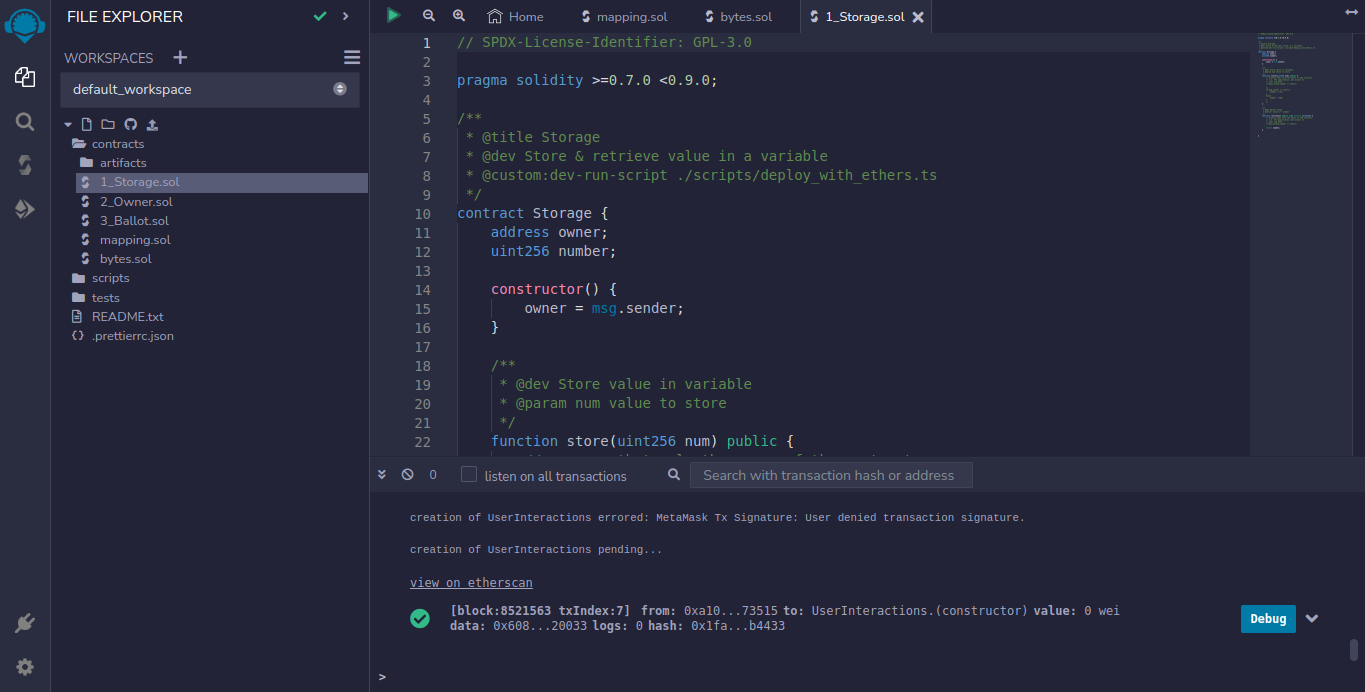
\includegraphics[width=1\textwidth]{img/Cap1/remix ide.png}
    \caption{Ambiente de Desenvolvimento Integrado Remix}
    \label{fig:remix}
\end{figure}
